\section{Resolução do Desafio}

\begin{minipage}{\linewidth}
  \centering
  \begin{minipage}{0.45\linewidth}
    Dado o circuito da \textbf{Figura \ref{fig:CircuitoDesafio}},
    considerar: $R_1 = 330\Omega$,
                $R_2 = 150\Omega$,
                $R_3 = 270\Omega$, \\
                $R_4 = 400\Omega$ e
                $R_5 = 100\Omega$.
    \begin{itemize}
      \item Identificar:
      \begin{itemize}
        \item os nós do circuito;
        \item a configuração de ligação dos componentes: série ou paralelo;
      \end{itemize}
      \item Calcular a resistência equivalente em cada ramo;
      \item Simplificar o circuito ao redesenhá-lo;
      \item Repetir o processo até obter a resistência equivalente total.
    \end{itemize}
  \end{minipage}
  \hspace{0.05\linewidth}
  \begin{minipage}{0.45\linewidth}
    \begin{figure}[H]
      \centering
      \caption{Circuito elétrico misto}
      \label{fig:CircuitoDesafio}
      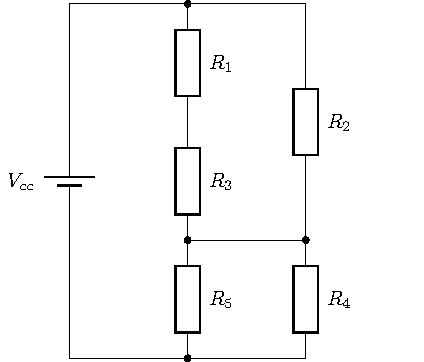
\includegraphics[scale=1.0]{fig-desafio}

      {\small Fonte: Próprio autor.}
    \end{figure}
  \end{minipage}
\end{minipage}






\subsection{Passo 1: Identificação dos nós}

\begin{minipage}{\linewidth}
  \centering
  \begin{minipage}{0.45\linewidth}
    Dados do circuito: \\
                $R_1 = 330\Omega$,
                $R_2 = 150\Omega$,
                $R_3 = 270\Omega$, \\
                $R_4 = 400\Omega$ e
                $R_5 = 100\Omega$.
  \end{minipage}
  \hspace{0.05\linewidth}
  \begin{minipage}{0.45\linewidth}
    \begin{figure}[H]
      \centering
      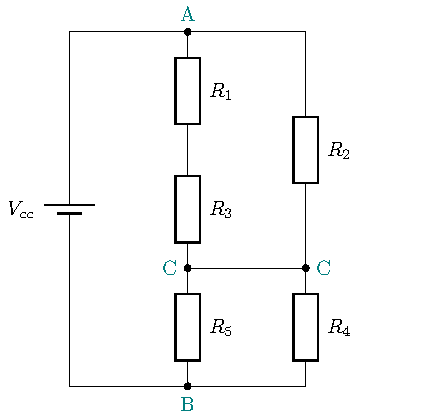
\includegraphics[scale=1.0]{fig-desafioPasso1}
    \end{figure}
  \end{minipage}
\end{minipage}










\subsection{Passo 2: Identificação de resistores em série}

\begin{minipage}{\linewidth}
  \centering
  \begin{minipage}{0.45\linewidth}
    Dados do circuito: \\
                $R_1 = 330\Omega$,
                $R_2 = 150\Omega$,
                $R_3 = 270\Omega$, \\
                $R_4 = 400\Omega$ e
                $R_5 = 100\Omega$.

      \begin{eqnarray}
        R_A & = & R_1 + R_3 \nonumber\\
        R_A & = & 330 + 270 \nonumber\\
        R_A & = & 600\Omega \nonumber
      \end{eqnarray}

  \end{minipage}
  \hspace{0.05\linewidth}
  \begin{minipage}{0.45\linewidth}
    \begin{figure}[H]
      \centering
      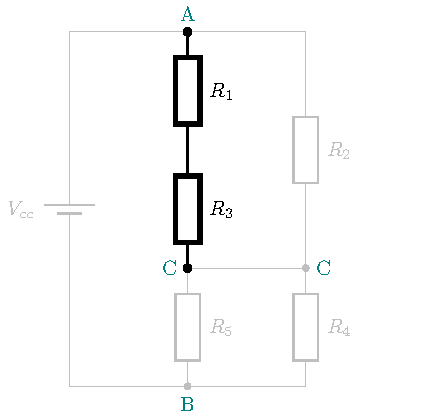
\includegraphics[scale=1.0]{fig-desafioPasso2}
    \end{figure}
  \end{minipage}
\end{minipage}







\subsection{Passo 3: Identificação de resistores em paralelo}

\begin{minipage}{\linewidth}
  \centering
  \begin{minipage}{0.45\linewidth}
    Dados do circuito: \\
                $R_1 = 330\Omega$,
                $R_2 = 150\Omega$,
                $R_3 = 270\Omega$, \\
                $R_4 = 400\Omega$ e
                $R_5 = 100\Omega$,\\
                $R_A = R_1 + R_3 = 600\Omega$.
       \begin{eqnarray}
         G_B & = & G_A + G_2 \nonumber\\
         R_B & = & R_A // R_2 \nonumber\\
         R_B & = & \frac{1}{\frac{1}{R_A} + \frac{1}{R_2} } \nonumber\\
         R_B & = & \frac{1}{\frac{1}{600} + \frac{1}{150} } \nonumber\\
         R_B & = & 120\Omega \nonumber
       \end{eqnarray}

  \end{minipage}
  \hspace{0.05\linewidth}
  \begin{minipage}{0.45\linewidth}
    \begin{figure}[H]
      \centering
      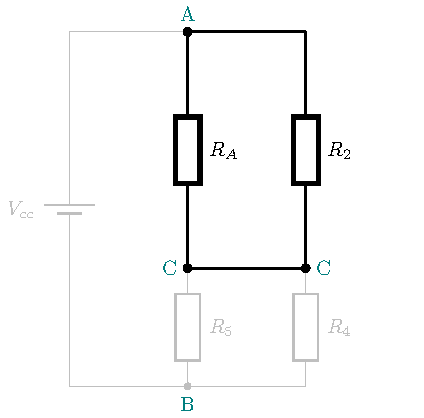
\includegraphics[scale=1.0]{fig-desafioPasso3}
    \end{figure}
  \end{minipage}
\end{minipage}








\subsection{Passo 4: Identificação de resistores em paralelo}

\begin{minipage}{\linewidth}
  \centering
  \begin{minipage}{0.45\linewidth}
    Dados do circuito: \\
                $R_1 = 330\Omega$,
                $R_2 = 150\Omega$,
                $R_3 = 270\Omega$, \\
                $R_4 = 400\Omega$ e
                $R_5 = 100\Omega$,\\
                $R_A = R_1 + R_3 = 600\Omega$, \\
                $R_B = R_A // R_2 = 120\Omega$.
        \begin{eqnarray}
         G_C & = & G_4 + G_5 \nonumber\\
         R_C & = & R_4 // R_5 \nonumber\\
         R_C & = & \frac{R_4 . R_5}{R_4 + R_5} \nonumber\\
         R_C & = & \frac{400 . 100}{400 + 100} \nonumber\\
         R_C & = & 80\Omega \nonumber
        \end{eqnarray}

  \end{minipage}
  \hspace{0.05\linewidth}
  \begin{minipage}{0.45\linewidth}
    \begin{figure}[H]
      \centering
      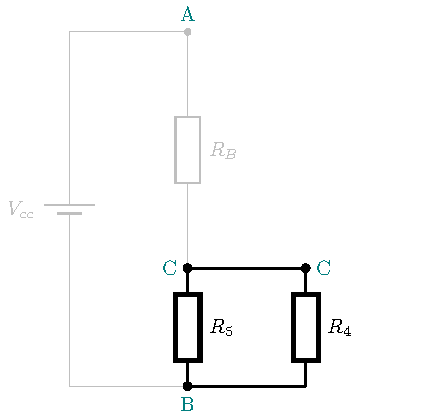
\includegraphics[scale=1.0]{fig-desafioPasso4}
    \end{figure}
  \end{minipage}
\end{minipage}






\subsection{Passo 5: Identificação de resistores em série}

\begin{minipage}{\linewidth}
  \centering
  \begin{minipage}{0.45\linewidth}
    Dados do circuito: \\
                $R_1 = 330\Omega$,
                $R_2 = 150\Omega$,
                $R_3 = 270\Omega$, \\
                $R_4 = 400\Omega$ e
                $R_5 = 100\Omega$,\\
                $R_A = R_1 + R_3 = 600\Omega$, \\
                $R_B = R_A // R_2 = 120\Omega$, \\
                $R_C = 80\Omega$.
        \begin{eqnarray}
          R_T & = & R_B + R_C \nonumber\\
          R_T & = & 120 + 80 \nonumber\\
          R_T & = & 200\Omega \nonumber
        \end{eqnarray}

  \end{minipage}
  \hspace{0.05\linewidth}
  \begin{minipage}{0.45\linewidth}
    \begin{figure}[H]
      \centering
      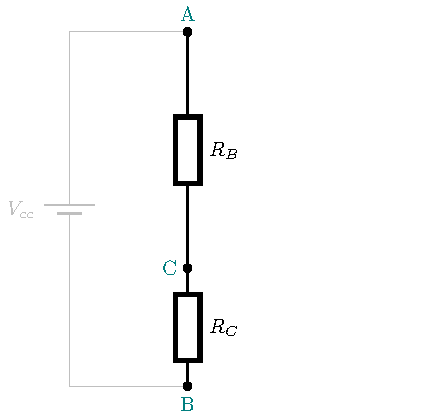
\includegraphics[scale=1.0]{fig-desafioPasso5}
    \end{figure}
  \end{minipage}
\end{minipage}



\subsection{Passo 6: Resistência Total do Circuito}

\begin{minipage}{\linewidth}
  \centering
  \begin{minipage}{0.45\linewidth}
    Dados do circuito: \\
                $R_1 = 330\Omega$,
                $R_2 = 150\Omega$,
                $R_3 = 270\Omega$, \\
                $R_4 = 400\Omega$ e
                $R_5 = 100\Omega$,\\
                $R_A = R_1 + R_3 = 600\Omega$, \\
                $R_B = R_A // R_2 = 120\Omega$, \\
                $R_C = 80\Omega$, \\
                $R_T = 200\Omega$.
  \end{minipage}
  \hspace{0.05\linewidth}
  \begin{minipage}{0.45\linewidth}
    \begin{figure}[H]
      \centering
      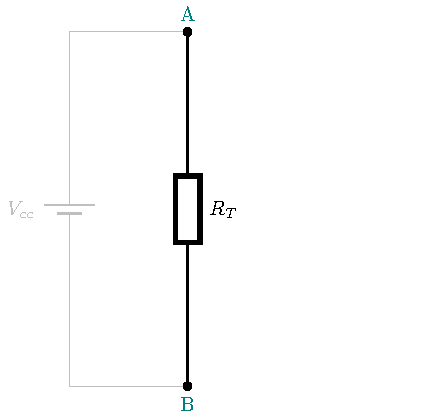
\includegraphics[scale=1.0]{fig-desafioPasso6}
    \end{figure}
  \end{minipage}
\end{minipage}
